% thesis.tex

\documentclass[12pt]{report}

\usepackage{utepcsthesis}
\usepackage{graphics}
\usepackage {tikz}
\usetikzlibrary {positioning}

\begin{document}

%%%%%%%%%%%%%%%%%%%%%
% Preliminary Pages %
%%%%%%%%%%%%%%%%%%%%%%%%%%%%%%%%%%%%%%%%%%%%%%%%%%%%%%%%%%%%%%%%%%%%%%%%%%%%%%%%

% Set the table of contents depth (tocdepth) to the least significant section
% type that you want to be included in the table of contents using this key:
%   1 = section
%   2 = subsection
%   3 = subsubsection
%   4 = paragraph
\setcounter{tocdepth}{2}

% The graduate school requires all caps for the title, and if
% the title contains more than one line, the lines should be
% of decreasing length, giving the look of an inverted pyramid.

\title{SECURE DATA PROVENANCE FOR IOT DEVICES}
% If the title is more than one line, separate the lines with \\[1pc]
% as shown below:
%\title{THIS IS THE VERY FIRST LINE\\[1pc]
%       THIS IS THE SECOND LINE\\[1pc]
%       THIS IS THE THIRD ONE}

% The author should also be all caps
\author{EBELECHUKWU NWAFOR}
% Uncomment to put degrees on title page
\AuthorDegrees{M.S.}
\date{FEB 2016}
\DeptName{Department of Computer Science}

\CommitteeChair{Gedare Bloom, Chair, Ph.D.}
%\CommitteeChair{Gedare Bloom, Chair, Ph.D.}
\CommitteeMembers{Wayne Patterson, Ph.D.}
                 {Gloria Washington, Ph.D.}
                 
%Uncomment if you have a fourth member on your committee
\AdditionalMember{Robert RubenGuira, Ph.D.}
				

\GradSchoolDean{Pablo Arenaz, Ph.D.}

%Produce the signature page
\makesigpage

%Uncomment if you want a copyright page
\begin{CenteredPage}
\copyright Copyright\\[0.2in]
by\\[0.2in]
Ebelechukwu Nwafor\\[0.2in]
2016
\end{CenteredPage}

%Delete if you don't want a dedication
\begin{CenteredPage}
{\it to my\\[0.2in]
MOTHER and FATHER\\[0.2in]
thanks for all the love and support, i am forever grateful}
\end{CenteredPage}
\maketitlepage

% acknowl.tex {Acknowledgements}

\addcontentsline{toc}{chapter}{Acknowledgements}

\chapter*{Acknowledgements}

 First and foremost, I would like to thank God for making this possible, without him i will not be where i am today. I would also like to thank my parents, Benneth and Chinwe for their constant encouragement, love and support.  \par I would like to thank my advisors Dr. Gedare Bloom and Dr. Legand Burge for their guidiance and encouragement.Also for believing in me and my research ideas. I would like to thank my lab partner Habbeeb Olufowobi and fellow graduate student Marlon Mejias for their constant constructive criticism and valuable input in various drafts revisions of my proposal.       % Acknowledgements, optional
%\include{preface}       % Preface, optional
% abstract.tex (Abstract)

\addcontentsline{toc}{chapter}{Abstract}

\chapter*{Abstract}
The concept of Internet of Things (IoT) offers immense benefits by
enabling devices to leverage networked resources thereby making more intelligent
decisions. The numerous heterogeneous connected devices that exist throughout
the IoT system creates new security and privacy concerns. Some of these concerns can
be overcome through data trust, transparency, and integrity, which can be
achieved with data provenance. Data provenance also known as data lineage provides a history of transactions that occurs on a data object from the time it was created to its current state.Data provenance has immense benefits in detecting and mitigating current and future vulnerability attacks and has applications in anomaly detection, access control, and digital forensics.  \par This dissertation looks at provenance with a focus on IoT devices. It takes a holistic approach in the creation, security and applications of provenance data. We create a provenance aware system for IoT devices. This ensure trust and helps establish causality for decisions and actions taken by an IoT connected system. As a result of the amounts of data that is generated from our data provenance system, there arises an issue of running out of memory.To address this issue,we look at prior work done in the area of data compression and graph summarization. We address this by proposing a novel data pruning technique.We conclude by looking at the applications of provenance for security of malicious attacks and anomaly detection of malicious threats.

      % Abstract, optional, but strongly recommended

\tableofcontents        % Generate Table of Contents

% If you a list of tables, uncomment the next line.
% It is required if the document contains three or more tables
%\listoftables

% If you use a list of figures, uncomment the next line
% It is required if the document contains three or more figures
%\listoffigures

% Here would go optional list of illustrations, maps, slides

%%%%%%%%
% Body %
%%%%%%%%%%%%%%%%%%%%%%%%%%%%%%%%%%%%%%%%%%%%%%%%%%%%%%%%%%%%%%%%%%%%%%%%%%%%%%%%

%Start arabic numbering, bottom of first page and top right of subsequent pages
\StartBody

\chapter{Introduction}\label{chapter:introduction}
The oxford English dictionary defines provenance as the place of origin or earliest known history of something. An example of provenance can be seen with a college transcript. A transcript can be defined as the provenance of a college degree because it outlines all of the courses satisfied in order to attain the degree.

\par In the field of computing, Data provenance also known as data lineage can be defined as the history of all transformations performed on a data object from the its creation to its current state. Data Provenance has been explored in the areas of scientific computing to etrack how an experiment is reproduced, in buisness to track the workflow processes,also in field of computer security for forensic analysis and intrusion detection.An example of provenance for software systems is a web server's log file. This file contains metadata for various request and response time and ip addresses of all host systems that tries to request information from the server. Provenance denotes the who, where and why of data.Provenance data is represented as an acyclic graph which denotes casual relationship and dependencies between entities.Provenance ensures trust and integrity of data. The information in which provenance offers can be used in digital forensics to investigate the cause of a malicious attack and also in intrusion detection system to further enhance the security of computing devices.  \textcolor{blue}{Most IoT devices are memory constrained devices} \textcolor{red}{TODO: Expand more on statement.}.

 
\textcolor{red}{TODO: Create transition from Data provenance to IoT...}


The internet of things(IoT) can be defined as a network of heterogeneous devices communicating together. With the recent data explosion,information is disseminated at every communication level that exists. From mobile devices to desktop computers and servers.Making IoT systems provenance aware is of the essence because it ensures trust and  integrity of systems. Enabling IoT device provenance aware allows devices to be able to capture information such as the who, where and how transformations occur on a data object enabling us to be able to trace back in the vent of a malicious attack.



\section{Motivation}
According to a report released by Cisco, it is estimated that a total of 50 million devices will be
connected to the internet by the year 2020. With the vast amounts of heterogeneous devices connected,
security and privacy risks are inceased. Rapid7, an  IT security and analytics organization, discovered that vulnerabilities exist in
baby monitors that allowed attackers unauthorized remote access to these devices
whereby an attacker can remotely view live video feeds. Having a provenance aware
system will be beneficial in this situation since we have a record of input and output
operations performed on the device, we can be able to look back on operations
performed on the device to determine who, where, and how a malicious activity
occurred. Devices (things) connected in an IoT network are embedded systems, which
require lightweight and efficient solutions compared with general purpose
systems.
This requirement is attributed to the constrained memory and computing of such
devices. A major issue arises in ensuring that data is properly secured and
disseminated across the IoT network. The vast amount of data generated from IoT
devices requires stronger levels of trust which can be achieved through data
provenance. Provenance has immense benefits in the IoT. Data provenance ensures
authenticity, integrity and transparency between information disseminated across an
IoT network. Security applications such as intrusion detection, digital forensics, and
access control can be further enhanced by incorporating data provenance in IoT
devices. The goal of data provenance is to determine causality and effect of actions or
operations performed on a data object. Provenance ensures transparency between things
connected in IoT systems. By creating data transparency, we can trace information to
determine where, if and when a malicious attack occurs. To achieve transparency, we
propose a secure provenance aware system that provides a detailed record of all data
transactions performed on devices connected in an IoT network and also investigate its applications of provenance data in providing intrusion detection to IoT devices.  \textcolor{red}{Data is generated in at a fast rate in real-time by sensors and actuators. The provenance of this data tends to be larger than the data itself.}

\section{Provenance-Aware IoT Device Use Case}

Consider a smart home which contains interconnected devices such as a thermostat connected which automatically sets the temperature of a room based on previous information of your desired temperature settings, a smart lock system that can be controlled remotely, a home camera motoring system, A smart fridge which allerts you when you are out of milk. A malicous intruder tries to gain access to the connected devices remotely. Provenance can be used to track the series  of events to determine where and how the malicious attack originated.It can also be used as a safeguard to alert of a possible remote or insider hijack thereby protecting us from future or current malicious attacks.

\begin{figure}[h]
\begin{center}

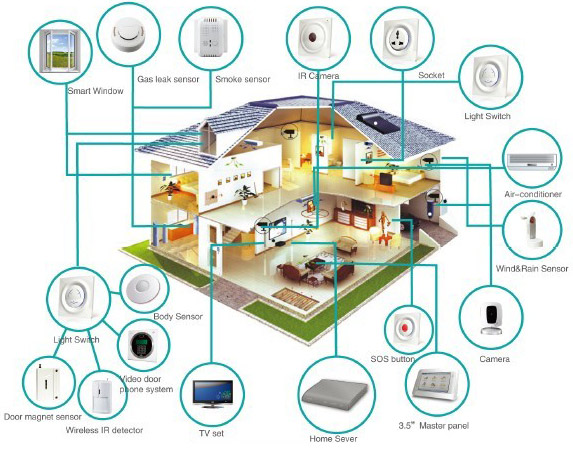
\includegraphics[height=3in]{smarthome-diagram.png}
\end{center}
\caption{Place holder for use case Diagram}

\end{figure}




\section{Research Questions}
collecting provenance data in IoT devices raises some key research issues. Some of these issues raised are outlined below:

\begin{itemize}

\item Memory constraints on IoT Devices: The vast amounts of data generated leads high storage space utilization . Proper memory management/data pruning techniques have to be employed for efficient storage of data on the memory contrained devices. 

\item How do we model provenance data for IoT devices? Do we use the OPM approach or create a taxonomy for modeling provenance data.

\item Provenance Query: How do we query tprovenance data in order to interprete provenance information and make anaylsis of data collected.

\item Provenance Versioning: Provenance version creates cycles. When a file is read or edited do we create a new instance of the file? Tracking all transformations that occurs on a data object in memeory constrained devices might lead to running out of storage space. A new instance of the provenance of that file should be created and included in the provenance data.

\item Securing Provenance: Due to the great level of sensitivity that  provenance data contains, we need to ensure the confidentiality and integrity of provenance data stored on IoT devices while at rest or in transit. Proper encryption and authentication techniques need to be employed to ensure confidentiality, integirty, and availability of provenance data.
\end{itemize}

\section{Research Contribution}

In this dissertation, we proposes the following key contributions:

\begin{itemize}
  \item A provenance collection framework which denotes causality and dependencies between entities contained in an IoT system.This system creates the groundwork for capturing and storing provenance data  on IoT devices.
  \item A novel framework for Data storage on embedded systems.This addresses the storage issues of the memory constrained IoT devices.
   \item A framework for providing intrusion detection using provenance data in an IoT system.
\end{itemize}

\section{Organization of Dissertation proposal}

The remaining portion of the dissertation proposal is organized as follows.  Chapter 2 talks about background information on data provenance, some of the techniques of collecting system level provenance, Data pruning techniques and also applications of data provenance with provenance based intrusion detection system. chapter 3 discusses our proposed provenance collection system  and focuses specifically on preliminary work done in creating a provenance aware system. Chapter 4 concludes the proposal and discusses the proposed framework and projected timeline for completion.

         % Introductory Chapter
% chap2.tex (Definitions)



\chapter{Related Work}\label{background}

This section outlines some of the state of the art in the area of data provenance collection systems, data compression techniques for data provenance, and models for representing provenance data.


\section{Related Work on Provenance Collection Systems}

There has been a considerable amount of work done on data provenance collection \cite{_general-purpose_2012, bates_trustworthy_2015, gessiou_towards_2012, muniswamy_reddy_provenance_2010}. Some of the work done has been focused on databases, sensor networks, scientific workflow systems and file system provenance but so far little attention has been given to provenance in IoT. Some of the prior work done on data provenance collection are outlined below:

\subsection{Provenance Aware Storage System(PASS)}
MuniswamyReddy
et al \cite{muniswamy_reddy} developed a provenance collection system that tracks  system\-level provenance of the Linux file system. Provenance information
is stored in the same location as the file system for easy accessibility, backup,
restoration, and data management. Provenance information is collected and stored in
the kernel space. PASS is composed of 3 major components: provenance collector, and provenance storage, provenance query. The collector keeps track of system level provenance. It intercepts system calls which are translated into provenance data and initially stored in memory as inode cache. Provenance data is then transferred to a file system in an kernel database, BerkleyDB. This database maps key value pairs for provenance data for fast index look up. PASS collects and stores provenance information containing a reference to the executable that created the provenance data, input files, a description of hardware in which provenance data is produced, OS information, process environment, process parameters, and other/data such as a random number generator seed. PASS detects and eliminates cycles that might occur in provenance dependencies as a result of version avoidance. Cycles violates the dependency relationships between entities. For example, a child node could depend on a parent node and also be an ancestor of a parent node. PASS eliminates cycles by merging processes that might have led to the cycles. It also provides functionality for querying provenance data in the database. The query tool is built on top of BerkleyDB. For querying provenance, users can process queries using the provenance explorer. Query is done using commands such as MAKEFILE  GENERATION which creates the sequence of events that led to the final state of a file or process. DUMP ALL, gets the provenance of the requested file. 

\subsection{HiFi}
Bates et al. \cite{hi_fi}  developed system level provenance collection framework for the Linux kernel using Linux Provenance Modules(LPM), this framework tracks system level provenance such as interprocess communication, networking, and kernel activities. This is achieved by mediating access to kernel objects. Linux Security Model is a framework that was designed for providing custom access control into the Linux kernel. It consists of a set of hooks which is executed before access decision is made. LSM was designed to avoid problem created by direct system call interception. The provenance information collected from the kernel space is securely transmitted to the provenance recorder in the user space. 
\par HiFi contains three components, provenance collector, provenance log and provenance handler. The collector and log are contained in the kernel space while the handler is contained in the user space. The log is a storage medium which transmits the provenance data to the user space. The collector contains the LSM which resides the kernel space. The collector records provenance data and writes it to the provenance log. The handler intercepts the provenance record from the log. This approach to collecting provenance data differs from our work since we focus on embedded systems and are concerned with input and output (I/O) data, which primarily involve sensor and actuator readings.

\subsection{RecProv}

RecProv \cite{rec_prov} is a provenance system which records user-level provenance, avoiding the overhead incurred by kernel level provenance recording. It does not require changes to the kernel like most provenance monitoring systems. It uses mozilla rr to perform deterministic record and replay by monitoring system calls  and non deterministic input. Mozilla rr is a debugging tool for linux browser. It is developed for the deterministic recording and replaying of the firefox browser in linux. Recprov uses PTRACE\_PEEKDATA from PTRACE to access the derefrenced address of the traced process from the registers. It also ensure the integrity of provenance data up till the point at which a host is compromised by trace isolation. Mozilla rr relies on PTRACE which intercepts system calls during context switching. It uses PTRACE to monitor the CPU state during and after a system call. It uses PTRACE\_PEEKDATA from PTRACE to access the derefrenced address of the traced process from the registers. System calls such as execve, clone, fork, open, read, write, clode, dup, mmap, socket, connect, accept are monitored which are used for file versioning. The provenance information generated is converted into PROV-JSON, a W3C standard for relaying provenance and also stored provenance data in Neo4j a graph database for visualization and storage of provenance graphs. 

\subsection{StoryBook}
Spillance et al \cite{story} developed a user space provenance collection system, Storybook, which allows for the collection of provenance data from the user space thereby reducing performance overhead. This system takes a modular approach; It allows the use of application specific extensions allowing additions such as database provenance, system provenance, and web and email servers. It achieves provenance capture by using FUSE for system level provenance and MySQL for database level provenance capture. StoryBook allows developers to implement provenance inspectors these are custom provenance models which captures the provenance of specific applications which are often modified by different application(e.g web servers, databases). When an operation is performed on a data object, the appropriate provenance model is triggered and provenance data for that data object is captured. StoryBook stores provenance information such as open, close, read or write, application specific provenance, causality relationship between entities contained in the provenance system. Provenance data is stored in key value pairs using Fable as the storage backend. Storybook allows for provenance query. It achieves this by looking up an inode in the ino hashtable.



\subsection{Trustworthy whole system provenance for Linux kernel}

Bates et al \cite{bates_towards_2013} provide a security model for provenance collection in the linux kernel. This is achieved by creating a Linux Provenance Model(LPM). LPM serves as a security layer which provides a security abstraction for provenance data. It is involved in the attestation disclosure of the application layer and authentication channel for the network layer. The goal of LPM is to provide an end to end provenance capture system. LPM ensures the following security guarantees: For LPM,the system must be able to detect and avoid malicious forgery of provenance data. The system must be trusted and easily verifiable. \par When an application invokes a system call, the LPM tracks system level provenance which is transmitted to the provenance module via a buffer . The provenance module registers contains hooks which records system call events. These events are sent to a provenance recorder in the user space. The provenance recorder ensures that the provenance data is stored in the appropriate backend of choice. Provence recorders offer storage support for Gzip, PostGreSQL, Neo4j and SNAP.



\subsection{Towards Automated Collection of Application-Level Data Provenance}
Tariq et \cite{tariq_towards_2012} all developed a provenance collection system which automatically collects interprocess provenance of applications source code at run time. This takes a different approach from system level provenance capture. It achieves provenance capture by using LLVM compiler framework and SPADE provenance management system. LLVM is a framework that allows dynamic compilation techniques of applications written in C, C++, Objective-C, and Java. Provenance is inserted during compilation. LLVM contains an LLVM reporter. This is a java class that parses the output file collected from the LLVM tracer and forwards the provenance data collected to the SPADE Tracer. SPADE is a provenance management tool that allows for the transformation of domain specific activity into provenance data. The LLVM Tracer module tracks provenance at the exit and entry of each function. The output is an Open Provenance Model in which functions are represented by an OPM process, arguments and return values are represented as an OPM artifact. To minimize provenance record, users are allowed to specify what functions they would like to collect provenance information at run time. The LLVM optimizer generates a graph of the target application. This graph is used to perform reverse reachability analysis  from the functions contained in the graph. A workflow of how the framework works in collecting provenance is as follows:

\begin{itemize}
\item The application is compiled and converted into bitcode using the LLVM C compiler, clang.

\item The LLVM Tracer module is compiled with bitcode.

\item Provenance instrumentation is added to the bitcode via the LLVM Trace module.

\item Instrumentation bitcode is converted into assembly code via the compiler llc

\item LLVM Tacer and Reporter is compiled into assembly code.

\item  The instrumented application and assembly code is compiled into an executable binary and sent to the SPADE kernel.
\end{itemize}

One major limitation to this approach of collecting application level provenance is that a user is required to have the source code of the specific application in which provenance data is required. Also, provenance collection is limited to function's exit and entry points.


\subsection{Provenance from Log Files: a BigData Problem}


Goshal et al \cite{ghoshal_provenance_2013} developed a framework for collecting provenance data from log files. They argue that log data contains vital information about a system and can be an important source of provenance information. Provenance is categorized based on two types: Process provenance and data provenance. Process provenance involves collecting provenance information of the process in which provenance is captured. Data provenance on the other hand describes the history of data involved in the execution of a process. Provenance is collected by using a rule based approach which consists of a set of rules defined in XML. The framework consists of three major components. The Rule engine which contains XML specifications for selecting, linking and remapping provenance objects from log files. The rule engine processes raw log files to structured Provence. There are three categories of rules as specified by the grammar. The match-set rules which selects provenance data based on a set of matching rules. Link Rules which specifies relationship between provenance events and Remap rules are used to specifying an alias for a provenance object. This component is integrated with the log processor. The Log processor component is involved with parsing log files with information contained in the rule engine. It converts every matching log information to a provenance graph representing entities(vertices) and their relationship(edges). The adapter converts the structured provenance generated by the Log processor into serialized XML format which is compatible with karma, a provenance service application that is employed for the storage and querying of the provenance data collected.




\subsection{Towards a Universal Data Provenance Framework using Dynamic Instrumentation}
Gessiou et al \cite{gessiou_towards_2012} propose a dynamic instrumentation framework for data provenance collection that is universal and does not incur the overhead of kernel or source code modifications. This is achieved by using DTrace, a dynamic instumentation utility that allows for the instrumentation of user-level and kernel-level code and with no overhead cost when disabled. It allows to be included at every point in time in a system  runtime without overhead issues from disabled probes.

The goal is to provide an easy extension to add provenance collection on any application regardless of its size or complexity. Provenance collection is implemented on the file system using PASS, on a database(SQLite) and a web browser(Safari). 
The logging component monitors all system calls for processes involved. The logging component contains information such as system-call arguments, return value, user id, process name, timestamp. The logging components includes functionalities to collect library and functional calls. The authors argue that applying data provenance to different layers of the software stack can provide varying levels of information. Provenance needs to be captured at the layer in which it is closest to the information that is needed to be captured. Provenance information that pertains to complex system activities such as a web browser or a database are collected. The information is collected from a process system-call and functional-call based on valid entry points contained in the process. DTrace dynamic instrumentation helps in discovering interesting paths in a system in which data propagates. This helps users use this information to collect a more accurate provenance data.


\subsection{Provenance-based trustworthiness assessment in sensor networks}
Lim et al. \cite{lim} developed a
model for calculating the trust of nodes contained in a sensor network by using data
provenance and data similarity as deciding factors to calculate trust. The value of
provenance signifies that the more similar a data value is, the higher the trust score.
Also, the more the provenance of similar values differ, the higher their trust score. The trust score of a system is affected by the trust score of the sensor that forwards data to the system. Provenance is determined by the path in which data travels through the sensor network. This work differs from our approach since the authors focus on creating a trust score
of nodes connected in a sensor network using data provenance and do not emphasize
how the provenance data is collected. We are focused on creating a
provenance aware system for I/O operations which is used to ensure trust of
connected devices. 

\subsection{Backtracking Intrusions}
Samuel et al \cite{King:2003:BI:945445.945467} developed a system, Backtracker, which generates an information flow of OS objects(e.g file, process) and events(e.g system call) in a computer system. From a detection point, information can be traced to pinpoint where a malicious attack occurred. The information flow represents a dependency graph which outlines the relationship between system events. Detection point is a point in which an intrusion was discovered. Time is included in the dependency between objects to reduce false dependencies. Time is denoted by an increasing counter. The time is recorded as the difference of when a system call is invoked till when it ends. Backtracker is composed of two major components: EventLogger and GraphGen. An EventLogger is responsible for generating system level event log for applications running on the system. EventLogger is implemented in two ways: using a virtual machine and also as a stand alone system. In a virtual machine, the application and OS is run within a virtual machine. The OS running inside of the virtual machine is known as the guest OS while the OS on the virtual machine is known as the host OS. The virtual machine alerts the EventLogger in the event that an application makes a system call and also when an application exits. EventLogger gets event information, object identities, dependency relationship between events from the virtual machine's monitor and also the virtual machine's physical memory. EventLogger stores the collected information as a compressed file. EventLogger can also be implemented as a stand alone system which is incorporated in an operating system. Virtual machine is preferred to a standalone system because of the use of virtual machine allows ReVirt to be leveraged. ReVirt enables the repay of instruction by instruction execution of virtual machines. This allows for whole information capture of workloads. After the information has been captured by the EventLogger, GraphGen is used to produce visualizations that outlines the dependencies between event and objects contained in the system. GraphGen also allows for pruning of data after it has been collected by the EventLogger. It contains regular expressions which are used to filter the dependency graph and prioritize important portions of the dependency graph.



\subsection{Provenance Recording for Services}
Grouth et al \cite{groth} developed a provenance collection system, PReServ which allows software developers to integrate provenance recording into their applications. They introduce P-assertion recording protocol as a way of monitoring process  documentation for Service Oriented Architecture(SOA) in the standard for grid systems. PreServ is the implementation of P-assertion recording protocol (PreP). PreP specifies how provenance can be recorded. PreServ contains a provenance store web service for recording and querying of p-assertions. P-assertions are provenance data generated by actors about the execution. It contains information about the messages sent and received as well as state of the message. PreServ is composed of three layers, the Message translator which is involved with converting all messages receive via HTTP request to XML format for the provenance store layer. It also determines which plug-in handle to route incoming request, the  Plug-Ins layer receives messages from the Message translator. It implements functionality that the Provenance Store component provides. This component allows third party developers to add new functionality to store provenance data without going through details of the code implementation. The backend component stores the P-assertions. Various backend implementations could be attached to the system by the plug-in component


\section{Related Work on Policy-based provenance data storage}

\subsection{Take Only What You Need: Leveraging Mandatory Access Control Policy to Reduce Provenance Storage Costs}

Bates et al \cite{Bates:2015:TOY:2814579.2814586} developed a system which allows maximizing provenance storage collection in the Linux OS environment using mandatory access control policy. this enables provenance avoidance of recording unnecessary provenance data and only recording interesting provenance that is important to an application. In MAC system, every object contains a label and the MAC policy specify interactions between different labels contained in the MAC. Provenance policy contains security context which is enforced by the MAC policy which contains permissions based on security context. IT provides the link between provenance and MAC. They argue that the system collects complete provenance without gaps in provenance relationship and still maintaining the MAC policy authorization domain. This is achieved by extending the work of Vijayakumar et. al.’s \cite{asiaccs12-vijayakumar} Integrity Walls project which allows mining SELinux policieswith the aim of finding Minimal Trusted Computing Base (MTCB) of various applications. A policy document is divided into trusted and untrusted labels. The trusted labels provides a thorough description of events relationship that can have access to the application. This information serves as a provenance policy that ensures a complete provenance relationship.

\subsection{A Provenance-aware policy language (cProvl) and a data traceability model (cProv) for the Cloud}

Ali et al \cite{Ali:2013:PPL:2569433.2569893} provides a provenance model, cProv, which illustrates relationships between entities contained in a cloud system. This model is build on PROV notation. cProv contains 5 derived nodes(cprov:cProcess, cprov:Resource, cProv:Transition, cprov:cResource, and cprov:pResource ). There are a total of 10 edges built on the relationships contained in the PROV notation. Node consists of properties such as location, time-to-live, virtual-to physical mappings, executed operations. They also develop a policy language, cProvl that allows for access of provenance data. cProvl is represented in XML and consists of rules  and conditions that expresses logic to enforce access of resources. Each rule contains an entity. XACML, a policy language for the enforcement of access control is used for implementing access control on the provenance policy information. cProvl is mapped to XACML to allow the policy to run on XACML which is widely used in the industry for access control implementation. An example of how the policy structure works is as follows: An application makes a request, this request is converted to the appropriate provenance aware request. This request is forwarded to the policy engine. The request is then evaluated by this layer by evaluating one or more policy rules as contained in a policy. This creates a response which is forwarded to the provenance converter which converted to the appropriate format for client utilization.



\section{Related Work on Data Compression}

\subsection{Secure Data Provenance Compression Using Arithmetic Coding in Wireless Sensor Networks(WSN)}

The authors \cite{hussain_secure_2014} encode the provenance of the path in which a sensor provenance travels using arithmetic coding, a data compression algorithm. Arithmetic coding assigns intervals to a string of characters by  cumulative probabilities of each character contained in the string. It assign probabilities by monitoring the activities of the WSN, this is known as the training phase. In this phase the number of times a node appears in a packet is counted. Each node in the WSN is regarded as a symbol. This is used as input to the arithmetic coding algorithm which generates a variable interval for the combination of symbols. For their application, provenance is referred to as the path in which data travels to the BS. The WSN contains a Base Station(BS) and a network of nodes. The base station is in charge of verifying the integrity of the packets sent. It is also where the encoded characters using arithmetic coding are decoded.  According to the authors, provenance is divided into two types: Simple provenance in which data generated from the leaf nodes and are forwarded to surrounding nodes towards the Base Station. In the other form of provenance, data is aggregated at an aggregation node and forwarded to a BS. Each node in the WSN is represented as a string of characters and is encoded using arithmetic coding. The BS is responsible for decoding encoded provenance information. Provenance is encoded at the respective nodes and forwarded to the next node in the sensor network. The BS recovers characters the same way they were encoded. It also receives the encoded interval to which it uses to decode characters by using the probability values saved in its storage.
















%\section{Intrusion Detection for IoT}



%%% Local Variables: 
%%% mode: latex
%%% TeX-master: "thesis"
%%% End:          % Chapter 2
% chap3.tex (Definitions and Theorem)

\chapter{Sensor Data Provenance Collection Framework for the IoT}

In this chapter, we define how provenance is collected and modeled along the IoT architectural stack. We also define implementation specifics of the provenance collection framework for IoT device. 

\section{IoT Provenance-Collection framework Information flow}
%This section discusses the data model in which we represent sensor and actuator reading of provenance data collected from IoT devices . It also talks about the relationship between IoT provenance Collection and PROV\-DM; How data is process and dissemenated accross the IoT architecture.
%
%\textcolor{red}{TODO: Talks about how we use PROV\-DM and what kinds of provenance we are looking to store}

A provenance model is used to represent causal relationship between objects and it is usually modeled as a Directed Acyclic Graph(DAG). This enables for better graphical representation of provenance relationships and also a unified format for representing provenance data. There are two major models for representing provenance, OPM and Prov-DM. PROV-DM is a predecessor and standardized version of OPM. It allows the modeling of data objects either physical or digital. PROV-DM is chosen as the model to represent provenance for our implementation because it allows for proper representation of all of the relationships in which we envision for IoT devices. This section defines a model for relaying provenance in IoT systems which is built on top of PROV-DM. 
From the IoT architecture as described in Section 2, we can see that data is disseminated from sensors and actuators across various layers contained in the IoT architectural stack. The provenance data produced from various sensors and actuators are collectively aggregated at the gateway layer and/or the cloud layer. We allow for provenance data to be translated to the appropriate PROV-DM format at the various levels of the IoT architecture. This allows offline processing of information at all layers of the IoT architecture even in the case of a network failure. Sensor readings are collected from devices as specified by a policy. This helps address the issue with memory constraint  of collecting provenance data in IoT devices. Policy specification and implementation are discussed in greater detail in chapter 4.  Figure 4.1 illustrates the provenance data aggregation that occurs at various layers of the IoT architectural stack.


\begin{figure}[h!]
\begin{center}

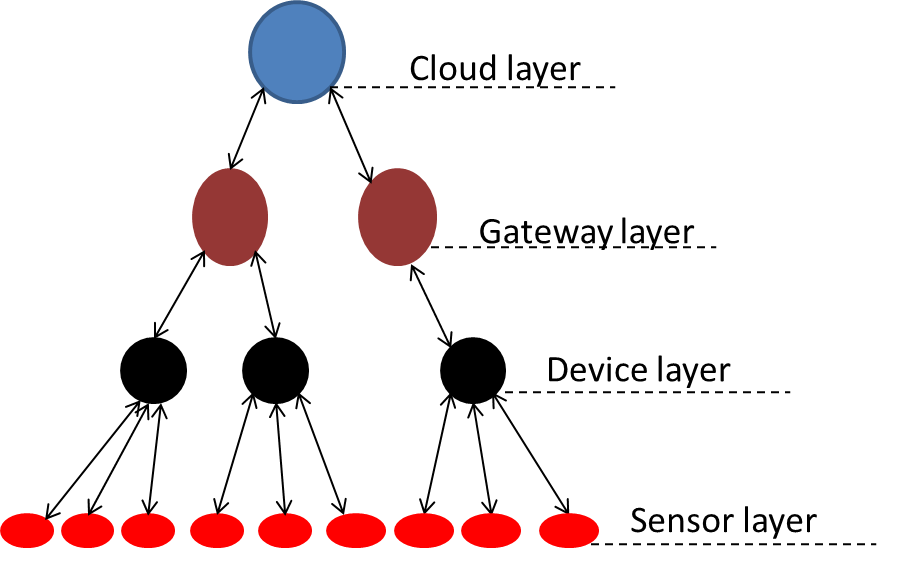
\includegraphics[width=3.0in]{iot.PNG}    
\end{center}
\caption{IoT provenance-collection data aggregation}
\label{autom}
\end{figure}


Using the scenario of a smart home use case as illustrated in chapter 2, a detailed example of how our provenance collection framework can be applied is described as follows:

\begin{itemize}

\item Provenance data is collected from sensor and actuator readings of devices contained in the smart home(e.g thermostat, refrigerator, and smart doors). The provenance data is collected as specified in a policy document. Policy document contains information of which provenance data to be collected in the device and can be only be defined by the device owner who serves as an administrator. 

\item Provenance data from multiple sensor and actuator readings is collected from each device is aggregated and passed along to the gateway. The information is transmitted to the cloud for storage in which further analysis could be conducted on the data to derive insights from the provenance data collected. This information is then transferred to the cloud where it is mapped using the PROV\-DM which allows for causal relationship between the objects contained in the IoT framework. Each layer in the provenance IoT architecture is independent of the and maintains provenance information that can be mapped using the PROV\-DM format which allows for the representation of dependencies that exists between objects contained in the device. This allows for provenance data to be further analyzed offline at the respective layers even in an event of network loss. 

\end{itemize}





\subsection{Provenance-Collection Model Definition}

It is assumed that provenance data is collected from the underlying IoT device using the framework outline in section 3 of this chapter below. Data is collected from sensors and actuators attached to an IoT device. The underlying construct is represented as a acyclic graph which denotes the relationship between multiple sensors and actuator readings. Since PROV-DM type provides a generic model for relaying provenance information, we define a more specific construct for representing provenance data in IoT devices based on  PROV-DM. In the context of IoT provenance, entity, process and agent are defined as follows:

\begin{itemize}

\item Agent: An agent contains information on an object that accesses an entity. Examples of agents in an IoT architecture are sensors, actuators, user roles(e.g admin). A unique identifier is given to each agents contained in the IoT framework.

\item Entity:  An entity can be defined as a data object that contains information which can be modified. An example entities are device files, processes, device memory contents.

\item Activity: An activity is a modification that an agent makes on an entity. An example of an activity are basic file access modifications such as read, write, delete, update. 


\end{itemize}


To better emphasize the provenance-collection model, an example of a use case for the provenance collection model is illustrated in the figure below.



\begin{figure}[h]
\begin{center}

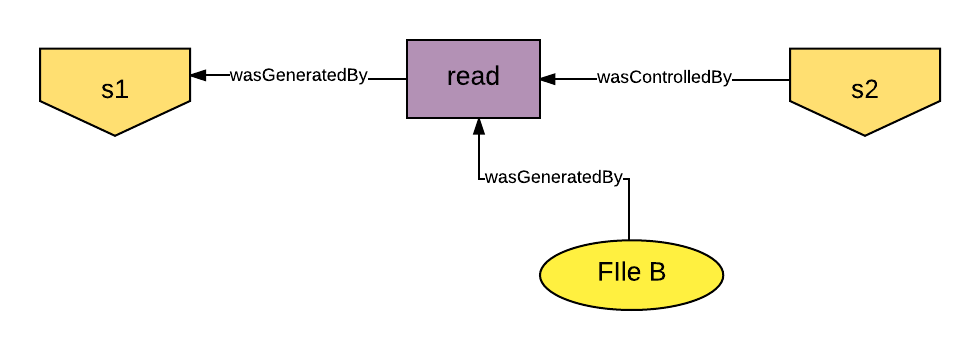
\includegraphics[width=4.0in]{provenance_model.png}    
\end{center}
\caption{Provenance-model use case}
\label{autom}
\end{figure}





The figure above depicts a dependency relationship between two sensors, s1 and s2. Consider the scenario of a smart home in which, s1 is smart thermostat contained in a smart home which regulates the temperature of the home and s2 is a sensor that detects the outside temperature. s1 constantly checks the temperature outside to regulate the temperature of the house accordingly. s1 tries to access information from s2. According to the provenance data model  definition, s1 and s2 are agents. The activity performed on s2 by s1 is read. File B is the entity in which s1 tries to read from s2 to determine the environmental temperature. The relationship between various components contained in the model is illustrated on the edges of the graph.

\par The relations define the relationship between types of a provenance model. We use the same instance of the relations contained in PROV-DM to represent relationships between types contained in the IoT framework.


\section{Provenance-Collection System}

In this section, we outline the components of our system and describe how provenance trace is collected across the IoT framework. Figure 1 displays the system architecture of our approach. Sensor and actuator readings in the form of Input and output(I/O) trace are recorded by the tracer component. This component intercepts system level I/O events and produces trace information in the Common Trace Format (CTF). CTF represents binary trace output information containing multiple streams of binary events such as I/O activity. Trace information is converted into the PROV-DM and serialized to PROV-JSON. This represents the relationship between provenance entities contained in the system. CTF conversion to OPM will be achieved using babeltrace. Babeltrace is a plugin which allows the ocnversion of CTF trace into various readable format. It includes plugins in which CTF trace data can be intercepted to create a custom conversion format. Our system relies heavily on data pruning to reduce and remove unimportant provenance in order to conserve memory and address the memory constraint issues faced by low memory embedded systems. This is achieved by using a policy-based approach in which a user with administrative privilege is given permission to create or modify a policy. This policy document dictates what provenance data to collect. Pruned provenance from the device is securely transmitted to a gateway and later transmitted and stored in a private cloud backend. The backend of choice is Neo4j, a graph database for efficient storage, query and visualization of provenance graph data.

\begin{figure}[h]
\begin{center}

\includegraphics[width =3.0in]{architecture.PNG}    
\end{center}
\caption{Proposed Model}
\label{architecture}
\end{figure}

The goal is to create a provenance\-aware system which records I/O operations on data for devices connected in an IoT system. For our implementation, several tools and hardware components are utilized in the development of our prototype, some of the tools utilized are outlined below:

\begin{itemize}
\item BeagleBone Black Board. This device is a microcontroller used to evaluate our approach. We choose the BeagleBone Board because it is a representation of what can be found on an IoT gateway device and it has the capability to include custom hardware in programmable logic. Also, BeagleBone is a low cost, simple IoT demonstrator that was chosen for its high performance, on­board emulation, and IoT gateway projects can be programmed without additional need for hardware tools.

%\item Real Time Executive for Multiprocessor Systems (RTEMS) is an open source real­time operating system (RTOS) for embedded systems. This operating system is a typical RTOS that may be deployed in IoT devices.

\item Neo4j, a graph database which allow the optimized querying of graph data. Since provenance represents causal dependencies, it is ideal to use a graph database to store the relationships between objects

\item lttng, a software tool for collecting system level trace on Linux system. 

\end{itemize}


\section{Experiment Evaluation}

I plan to evaluate the effectiveness of my approach for provenance collection by using an intrusion detection system specifically developed for IoT. An IDS is used to detect malicious attacks based on certain policy or threshold set by an administrator. There are two types of  IDS: rule-based/Signature-based approach, or anomaly-based approach. Signature-based approach allows for intrusion monitoring by specific known signatures of malicious attacks. An example of a signature-based IDS is an anti-virus software. On the other hand, anomaly-based IDS monitors intrusion by patterns that falls out of the normal system function. Most anomaly-based approach deals with the use of machine learning to classify normal or anomalous behavior. This can be useful to detect unknown malicious attacks. Provenance collection IDS system uses provenance data to provide intrusion detection capabilities in an IoT framework. It follows a Signature-based approach in which provenance data collected from the IoT framework is used for intrusion detection. 
\par The IDS is developed using the work of Xie et al \cite{Xie:2016:UID:2936026.2936232}. Xie et al proposes an intrusion detection system, Provenance-aware Intrusion Detection and Analysis System(PIDAS) which uses system-level provenance data to provide real-time vulnerability intrusion detection on system behaviors. The system collects provenance from system calls, detects intrusion and analyzes vulnerabilities that exists based on provenance data. PIDAS system contains three essential components: the collector which records provenance information of applications running in the user space. Provenance data is stored in a key-value pair database for easy query of acyclic graphs. The detector extracts dependency relationships from the provenance data and stores this information in a repository for further analysis. The analyzer is responsible for identifying all other intrusion activities that might occurred. It achieves this by making queries to view all dependencies from the detected intrusion point. Provenance detector is made possible by using a provenance-based algorithm that matches the path contained in the graph.


The detector consists of three steps. Rule-buit which collects normal system behavior of provenance data and stores this information in a ruleDB. A ruleDB consists of a key-value pair which has parent and child relationship in the dependency graph. The rule-built is used to match observed provenance events  to detect system intrusion. Provenance information in the form of dependency relationships is matched with the child/parent dependency rule information contained in the ruleDB. This information is used to compute the decision value which determines if there has been an intrusion.  A description of the rule matching and scoring algorithm is described in detail below: 

\begin{itemize}

\item provenance data is divided into dependency relationships, $Dep_1,...,Dep_n. Dep_i =(A, B)$. Where A is the parent of B

\item The algorithm checks if there exists a match in the path between edges contained in the provenance dependency database, ruleDB. If there exists a path, a score of 1 is given to the path. This score is known as the path dubiety. Otherwise, if the path does not match any edge in the ruleDB, a score of 0 is given to the path.

Let R = provenance information of a program and G = provenance information contained in ruleDB. For each $Dep_i = (A, B) \in R, if Dep_i = (A, B) \in G$. intrusion dubiety = 1 else set intrusion dubiety = 0

\item The path decision, P is the sum of the dubiety of all the edges contained in the provenance data divided by the number of paths contained in the provenance dependency database.

 \[P =\frac{\sum\limits_{i=1}^W dubeity of Dep_i }{W} \] This information is compared with a threshold value, T. If P $>$ T, an anomaly exists in the system.

\end{itemize}

I plan to compare the integration of our provenance collection framework and storage efficiency framework with PIDAS to a baseline which consists of the PIDAS system without the integration of our proposed framework. More specifically, I plan to evaluate the false negative and false positive rate for the IDS system as compared to the baseline. False positive dictates the number of times in which an intrusion has been wrongly detected. This signifies that a path contained in an applications provenance was detected and not found in the ruleDB. On the other hand, false negative rate identifies the number of times a intrusion has not been detected. I also plan to evaluate the throughput of the system with the proposed baseline.





%\section{Provenance Aware IDS System for IoT }
%
%This section outlines the core functionalities of our model PAIST. 
         % Chapter 3
% chap4.tex (Definitions and Theorem)

\chapter{Solving Most Narrow-Interval Linear Systems Is Easy: Known
Result} \label{MostNarrowEasy}

In this chapter we will define what we mean by {\em narrow intervals\/} and
present a positive result concerning systems of interval linear equations
having such narrow intervals.  This result was first discovered by Lakeyev
and Kreinovich in the mid 1990's.

\section{Definitions}

\begin{definition}
{\rm We say that the number $\tilde x$ represents a number $x$ with
{\em absolute accuracy\/} $\Delta>0$ if $|x-\tilde x|\leq\Delta$.}
\end{definition}

\begin{definition}
{\rm By {\em absolute half-width\/} of the interval ${\bf x}=[x^-,x^+]$, we
mean the smallest number $\Delta>0$ for which every number in ${\bf x}$ is
represented with an absolute accuracy~$\Delta$ by $\tilde x=\displaystyle{
\frac{x^-+x^+}{2}}$.\\[0.5pc]
{\bf Proposition} It can be seen that the absolute half-width of ${\bf x}$ is
$$
  \max_{x\in [x^-,x^+]} |x-\tilde x| = \frac{x^+-x^-}{2}.
$$}
\end{definition}

\begin{definition}
{\rm By {\em absolute width\/} $W$ of an interval ${\bf x}=[x^-,x^+]$, we mean
twice the absolute half-width of ${\bf x}$, i.e.,
$$
  W([x^-,x^+])=x^+-x^-.
$$}
\end{definition}

\begin{definition}
{\rm We say that an interval ${\bf x}$ is {\em $\Delta$-narrow in the sense
of absolute accuracy\/} if $W({\bf x})\leq\Delta$.}
\end{definition}

\begin{definition}
{\rm Let $\varepsilon>0$ be a real number, let $D\subseteq R^N$ be a closed
and bounded set of positive $N$-dimension volume $V(D)>0$, and let
$P(x)$ be a property that is true for some points $x\in D$.  We say that $P(x)$
is true for {\em $(D,\varepsilon)$-almost all\/} $x$ if}
$$
  \frac{V(\{x\in D|\neg P(x)\})}{V(D)}\leq \varepsilon.
$$
\end{definition}

\begin{definition}
{\rm Let $\eta>0$ be a real number.  We say that intervals
$$
  [r_1-d_1,r_1+d_1],\ldots,[r_n-d_n,r_n+d_n]
$$
are {$\eta$-close} to intervals
$$
  [\tilde x_1-\Delta_1,\tilde x_1+\Delta_1],\ldots,[\tilde x_n-\Delta_n,
   \tilde x_n+\Delta_n]
$$
if $|r_i-\tilde x_i|\leq\eta$ and 
$|d_i-\Delta_i|\leq\eta$ for all $i$.}
\end{definition}

\begin{definition}
{\rm Let $\cal U$ be an algorithm that solves some systems of interval linear
equations, and let $\eta>0$ be a real number.  We say that an algorithm 
$\cal U$ is {\em $\eta$-exact\/} for the interval matrices ${\bf a}_{ij}$ and
${\bf b}_i$ if for every interval matrix ${\bf a}_{ij}^\prime$ and 
${\bf b}_i^\prime$ that are $\eta$-close to ${\bf a}_{ij}$ and ${\bf b}_i$,
the algorithm $\cal U$ returns the exact solution to the system}
$$
  \sum_{j=1}^n {\bf a}_{ij}^\prime x_j = {\bf b}_i^\prime.
$$
\end{definition}

\begin{definition}
{\rm We say that an algorithm $\cal U$ is {\em almost always exact for narrow 
input intervals\/} if for every closed and bounded set $D\subseteq R^N
(N=n\cdot m+n)$ there exist $\varepsilon>0$, $\Delta>0$ and $\eta>0$ such
that, for $(D,\varepsilon)$-almost all $\tilde a_{ij}$ and $\tilde b_i$, if
all input intervals ${\bf a}_{ij}$ and ${\bf b}_i$
(containing $\tilde a_{ij}$ and $\tilde b_i$ respectively)
are $\Delta$-narrow (in the sense of absolute accuracy), then the
algorithm $\cal U$ is $\eta$-exact for ${\bf a}_{ij}$ and ${\bf b}_i$.}
\end{definition}

\section{Theorem}

\begin{theorem} \label{almost-all-theorem}
There exists a feasible (polynomial-time) algorithm $\cal U$ that is almost 
always exact for narrow input intervals.
\end{theorem}

\medskip

\noindent
This theorem was proven in 1995 by Lakeyev and Kreinovich
(see~\cite{Lakeyev1995}).

\section{Open Problem}
Theorem \ref{almost-all-theorem} says that we can have a feasible algorithm 
that solves {\em almost all\/} narrow-interval linear equation systems, but 
it does not say whether we can solve {\em all\/} of them in reasonable time.  
Thus, there still remains an open question:

\begin{quote}
{\it Can a feasible algorithm be developed for the general problem of
solving systems of linear equations with narrow-interval coefficients?}
\end{quote}

\noindent
The answer to this open question is the main concern of this thesis.

We will show that the problem of solving all narrow-interval linear equation
systems is NP-hard; moreover, we will show that the problem is NP-hard not
only for intervals that are narrow in the sense of absolute accuracy, but
also in the sense of relative accuracy.

         % Chapter 4
% chap5.tex (Definitions, Theorem and Proof)

\chapter{Solving Narrow-Interval Linear Systems Is
NP-Hard: New Result} \label{NewResult}

In this chapter we present the main result upon which this thesis is
centered---a new theorem and a proof for it based upon the
reduction\footnote{The reduction used is called a {\em polynomial-time
one-one reduction}, a special case of polynomial-time many-one reductions.}
of a system of (arbitrary) interval linear equations to a system of
narrow-interval linear equations.

\section{Definitions}

\begin{definition}
{\rm We say that the (non-zero) number $\tilde x$ represents a number $x$ with
a {\em relative accuracy\/} $\delta>0$ if $\displaystyle{\frac{|x-\tilde x|}
{|\tilde x|}}\leq\delta$.}
\end{definition}

\begin{definition}
{\rm By {\em relative half-width\/} of the interval ${\bf x}=[x^-,x^+]$
where $0\not\in[x^-,x^+]$, we
mean the smallest number $\delta>0$ for which every number in ${\bf x}$ is
represented with a relative accuracy~$\delta$ by $\tilde x=\displaystyle{
\frac{x^-+x^+}{2}}$.\\[0.5pc]
{\bf Proposition} It can be seen that the relative half-width of ${\bf x}$
where $0\not\in[x^-,x^+]$ is}
$$
  \max_{x\in [x^-,x^+]}\frac{|x-\tilde x|}{|\tilde x|}=
   \frac{x^+-x^-}{2|\tilde x|}.
$$
\end{definition}

\begin{definition}
{\rm By {\em relative width\/} $W^{rel}$ of an interval ${\bf x}=[x^-,x^+]$
where $0\not\in[x^-,x^+]$,
we mean twice the relative half-width of ${\bf x}$, i.e.,
$$
  W^{rel}([x^-,x^+])=\frac{x^+-x^-}{|\tilde x|}.
$$}
\end{definition}

\begin{definition}
{\rm We say that an interval ${\bf x}$ is {\em $\delta$-narrow in the sense 
of relative accuracy\/} if $W^{rel}({\bf x})\leq\delta$.}
\end{definition}

\begin{definition}
{\rm We say that an interval ${\bf x}$ is {\em $\delta$-narrow\/} if it is
both $\delta$-narrow in the sense of absolute accuracy and $\delta$-narrow in
the sense of relative accuracy.}
\end{definition}

\section{Theorem}
\begin{theorem}
For every $\delta>0$, the problem of solving systems of interval linear
equations with $\delta$-narrow intervals is computationally intractable
(\/{\rm NP}-hard).
\end{theorem}

\begin{corollary}
For every $\Delta>0$, the problem of solving systems of interval linear
equations with intervals $\Delta$-narrow in the sense of absolute accuracy 
is computationally intractable (\/{\rm NP}-hard).
\end{corollary}

\begin{corollary}
For every $\delta>0$, the problem of solving systems of interval linear
equations with intervals $\delta$-narrow in the sense of relative accuracy is
computationally intractable (\/{\rm NP}-hard).
\end{corollary}

\newpage
\section{Proof}

\subsection{Part I: Reduction of Interval Linear System to Narrow-Interval
Linear System}

We have seen that the general problem of solving interval linear equation
systems (\ref{d1}) is NP-hard.  We now intend to show that this general
problem can be reduced to the problem of solving a system of 
interval linear equations with $\delta$-narrow intervals.

Let us start with an arbitrary interval linear equation system (\ref{d1}).  To
reduce it to a $\delta$-narrow interval linear equation system, we introduce
new variables $w_i$, $y_{ij}$ and $z_{ij}$ for all $i=1,\ldots,m$ and
$j=1,\ldots,n$.  For the enlarged list of $m+n+2mn$ variables (i.e., $x_j$,
$w_i$, $y_{ij}$ and $z_{ij}$) we introduce the following new system of
$m+n+2mn$ $\delta$-narrow interval linear equations\footnote{For clarity,
non-interval coefficients can be thought of as intervals of zero width; e.g., 
the coefficient for each variable $y_{ij}$ is $[1,1]$ and each coefficient 
$c_i$ is equivalent to the interval $[c_i,c_i]$.}:
\begin{eqnarray}
  \sum_{j=1}^n y_{ij} +
   \sum_{j=1}^n [1-\frac{\delta}{2},1+\frac{\delta}{2}]z_{ij} +
   [1-\frac{\delta}{2},1+\frac{\delta}{2}]w_i &=& c_i, \label{p1a}\\
  w_i &=& \gamma_i, \label{p1b}\\
  y_{ij} - \mu_{ij} x_j &=& 0, \label{p1c}\\
  z_{ij} - \nu_{ij} x_j &=& 0, \label{p1d}
\end{eqnarray}
where $\delta>0$ and the numerical (non-interval) coefficients $c_i$,
$\gamma_i\geq 0$, $\mu_{ij}$ and $\nu_{ij}\geq 0$ will be chosen in such a
way that for every solution of this $\delta$-narrow interval linear equation
system (\ref{p1a})--(\ref{p1d}) we have
\begin{equation}
  c_i - [1 - \frac{\delta}{2}, 1 + \frac{\delta}{2}] w_i =
   [b_i^-, b_i^+] \label{p2}
\end{equation}
and
\begin{equation}
  y_{ij} + [1 - \frac{\delta}{2}, 1 + \frac{\delta}{2}] z_{ij} =
   [a_{ij}^-, a_{ij}^+] x_j \label{p3}
\end{equation}
for all $i=1,\ldots,m$ and $j=1,\ldots,n$.

Let us first find the values for $c_i$ and $\gamma_i$.  From equation
(\ref{p1b}) we know that $w_i = \gamma_i$.  By substituting this expression
into equation (\ref{p2}) we get
$$
  c_i - [1 - \frac{\delta}{2}, 1 + \frac{\delta}{2}] \gamma_i =
   [b_i^-, b_i^+]. \label{p4}
$$
Intervals are equal {\em if and only if\/} their endpoints coincide.  Since we
are looking for a solution with $\gamma_i\geq 0$, the equations for the
endpoints take the following forms:
\begin{equation}
  c_i - (1 - \frac{\delta}{2}) \gamma_i = b_i^+ \label{p5}
\end{equation}
and
\begin{equation}
  c_i - (1 + \frac{\delta}{2}) \gamma_i = b_i^-. \label{p6}
\end{equation}
Subtracting the second equation from the first we get
$$
  \delta\cdot\gamma_i = b_i^+ - b_i^-,
$$
and hence,
\begin{equation}
  \fbox{${\displaystyle\gamma_i=\frac{1}{\delta}(b_i^+-b_i^-).}$} \label{GAMMA}
\end{equation}
Substituting this value into equation (\ref{p5}), we get
$$
  c_i - (1 - \frac{\delta}{2}) \frac{1}{\delta}(b_i^+ - b_i^-) = b_i^+
$$
from which we get
$$
  c_i - (\frac{1}{\delta} - \frac{1}{2}) (b_i^+ - b_i^-) =  b_i^+,
$$
and hence,
\begin{equation}
  \fbox{${\displaystyle c_i=\frac{1}{2}(b_i^++b_i^-)
   +\frac{1}{\delta}(b_i^+-b_i^-).}$}                                 \label{C}
\end{equation}

Now let us find the values for $\mu_{ij}$ and $\nu_{ij}$.  From
equations (\ref{p1c}) and (\ref{p1d}) we conclude that $y_{ij}=\mu_{ij}x_j$
and $z_{ij}=\nu_{ij}x_j$.  Substituting these expressions into equation
(\ref{p3}) we get
$$
  \mu_{ij} x_j + [1-\frac{\delta}{2},1+\frac{\delta}{2}] \nu_{ij} x_j =
   [a_{ij}^-, a_{ij}^+] x_j.
$$
For this equality to be true for all $x_j$, coefficients for $x_j$ on both
sides of the equation must coincide.  Thus, we conclude that
$$
  \mu_{ij} + [1 - \frac{\delta}{2}, 1 + \frac{\delta}{2}] \nu_{ij} =
   [a_{ij}^-, a_{ij}^+].
$$
As stated before, for intervals to be equal their endpoints must coincide,
and since we are looking for a solution for $\nu_{ij}\geq 0$, the equations
for the endpoints take the following forms:
\begin{equation}
  \mu_{ij} + (1 + \frac{\delta}{2}) \nu_{ij} = a_{ij}^+ \label{p8}
\end{equation}
and
\begin{equation}
  \mu_{ij} + (1 - \frac{\delta}{2}) \nu_{ij} = a_{ij}^-. \label{p9}
\end{equation}
Subtracting the second equation from the first we get
$$
  \delta\cdot\nu_{ij} = a_{ij}^+ - a_{ij}^-,
$$
and hence,
\begin{equation}
  \fbox{${\displaystyle\nu_{ij}=\frac{1}{\delta}(a_{ij}^+-a_{ij}^-).}$}
                                                                     \label{NU}
\end{equation}
Substituting this value back into equation (\ref{p8}) we get
$$
  \mu_{ij} + (1 + \frac{\delta}{2}) \frac{1}{\delta}(a_{ij}^+ - a_{ij}^-) =
   a_{ij}^+
$$
which leads to
$$
  \mu_{ij}+(\frac{1}{\delta}+\frac{1}{2})(a_{ij}^+ - a_{ij}^-) = a_{ij}^+,
$$
and hence,
\begin{equation}
  \fbox{${\displaystyle\mu_{ij}=\frac{1}{2}(a_{ij}^++a_{ij}^-)
   -\frac{1}{\delta}(a_{ij}^+-a_{ij}^-).}$}                          \label{MU}
\end{equation}

\newpage
\subsection{Part II: The Two Systems Are ``Equivalent''}

Let us show that every system (\ref{d1}) of interval linear equations is
``equivalent'' to the $\delta$-narrow interval linear equation system
(\ref{p1a})--(\ref{p1d}) in the following sense:
\begin{description}
  \item[Claim 1] If $(x_1,\ldots,x_n)$ is a solution of the original system
    (\ref{d1}), then for the same values $x_1,\ldots,x_n$, and for some values
    $w_1,\ldots,w_m$, $y_{11},\ldots,y_{mn}$ and $z_{11},\ldots,z_{mn}$, the 
    extended tuple
    \begin{equation}
       (x_1,\ldots,x_n,w_1,\ldots,w_m,y_{1 1},\ldots,y_{m n},
        z_{1 1},\ldots,z_{m n}) \label{extsolution}
    \end{equation}
    is a solution of the $\delta$-narrow interval system
    (\ref{p1a})--(\ref{p1d}).
  \item[Claim 2] Conversely, if tuple (\ref{extsolution}) is a solution of the
    $\delta$-narrow interval linear equation system (\ref{p1a})--(\ref{p1d}),
    then $(x_1,\ldots,x_n)$ is a solution of the original system (\ref{d1})
    for the same values $x_1,\ldots,x_n$.
\end{description}
We will now prove that the two systems are indeed ``equivalent'' in the above
sense.

\subsubsection{Proof of Claim 1}
Let us assume that ($x_1,\ldots,x_n$) is a solution of the
original system (\ref{d1}).  By definition, 
if $(x_1,\ldots,x_n)$ is a solution to the original system (\ref{d1}), then
there must exist values $a_{ij}\in[a_{ij}^-,a_{ij}^+]$ and
$b_i\in[b_i^-,b_i^+]$ such that
\begin{equation}
  \sum_{j=1}^n a_{ij} x_j = b_i \label{claim1}
\end{equation}
for all $i=1,\ldots,m$.  With this in mind, let us introduce new parameters
$\alpha_{ij}=a_{ij}-a_{ij}^-$ and $\beta_i=b_i-b_i^-$; thus, $a_{ij}=a_{ij}^-+
\alpha_{ij}$ and $b_i=b_i^-+\beta_i$.  Substituting these expressions into
(\ref{claim1}) we get
\begin{equation}
  \sum_{j=1}^n (a_{ij}^-+\alpha_{ij}) x_j = b_i^-+\beta_i. \label{newsolution}
\end{equation}
Since $a_{ij}\in[a_{ij}^-,a_{ij}^+]$, we conclude that 
$\alpha_{ij}\in[0,a_{ij}^+-a_{ij}^-]$.  Similarly, since
$b_i\in[b_i^-,b_i^+]$, we conclude that $\beta_i\in[0,b_i^+-b_i^-]$.

Now let us show that there exists an extended tuple (\ref{extsolution}) that is
a solution to system (\ref{p1a})--(\ref{p1d}) for the same values
$x_1,\ldots,x_n$ and for appropriately chosen values of $w_1,\ldots,w_m$,
$y_{11},\ldots,y_{mn}$ and $z_{11},\ldots,z_{mn}$.  In order to have equations
(\ref{p1b})--(\ref{p1d}) automatically satisfied, we will take $w_i=\gamma_i$,
$y_{ij}=\mu_{ij}x_j$ and $z_{ij}=\nu_{ij}x_j$.  It is thus sufficient to show
that equation (\ref{p1a}) is satisfied for all $i=1,\ldots,m$; in other words,
we need to show that there exist values
${\displaystyle\kappa_i\in[1-\frac{\delta}{2},1+\frac{\delta}{2}]}$ and
${\displaystyle\lambda_{ij}\in[1-\frac{\delta}{2},1+\frac{\delta}{2}]}$ such
that
\begin{equation}
  \sum_{j=1}^n y_{ij}+\sum_{j=1}^n\lambda_{ij}z_{ij}+\kappa_i w_i=c_i
   \label{s1a}
\end{equation}
for all $i=1,\ldots,m$.

Note that for any given $i$, if $\gamma_i=0$ (and thus $w_i=0$), then
$\kappa_i w_i=0$, implying that $\kappa_i$ can be {\em any value\/} as long as
${\displaystyle\kappa_i\in[1-\frac{\delta}{2},1+\frac{\delta}{2}]}$ (e.g., 
$\kappa_i=1$).  Likewise, for any given $i$ and $j$, if $\nu_{ij}=0$ (and thus 
$z_{ij}=0$), then  $\lambda_{ij}z_{ij}=0$, implying that $\lambda_{ij}$ can be 
{\em any value\/} as long as ${\displaystyle\lambda_{ij}\in[1-\frac{\delta}{2},
1+\frac{\delta}{2}]}$ (e.g., $\lambda_{ij}=1$).  Therefore, for the remainder
of the proof we will be choosing $\kappa_i$ only for those $i$ for which
$\gamma_i>0$ (i.e., $b_i^-<b_i^+$), and we will be choosing $\lambda_{ij}$ 
only for those $i$ and $j$ for which $\nu_{ij}>0$ (i.e., $a_{ij}^-<a_{ij}^+$).

We have chosen $w_i$ and $c_i$ for which the equation (\ref{p2}) is true,
i.e., for which
$$
  c_i - [1 - \frac{\delta}{2}, 1 + \frac{\delta}{2}] w_i = [b_i^-, b_i^+].
$$
Crudely speaking, this equality means that when we take different values for
$\kappa_i$ such that
$\kappa_i\in[1-{\displaystyle\frac{\delta}{2}},1+{\displaystyle\frac{\delta}
{2}}]$, the set
$$
  c_i - [1 - \frac{\delta}{2}, 1 + \frac{\delta}{2}] w_i
$$
of possible values of $c_i-\kappa_i w_i$ coincides with the interval
$[b_i^-, b_i^+]$.  In particular, since $b_i\in[b_i^-,b_i^+]$, there must
exist a value $\kappa_i\in[1-{\displaystyle\frac{\delta}{2}},1+{\displaystyle
\frac{\delta}{2}}]$ for which
$$
  c_i-\kappa_i w_i = b_i = b_i^- + \beta_i.
$$
From this equation we can find the exact value of $\kappa_i$.

We know from equation (\ref{p1b}) that $w_i=\gamma_i$, so by substitution we
get
$$
  c_i - \kappa_i \gamma_i = b_i^- + \beta_i,
$$
and hence,
$$
  \kappa_i=\frac{1}{\gamma_i}(c_i-b_i^--\beta_i).
$$
Substituting the values of $\gamma_i$ and $c_i$ from equations (\ref{GAMMA})
and (\ref{C}) we get
$$
  \kappa_i=\frac{\delta}{b_i^+-b_i^-}(\frac{1}{2}(b_i^++b_i^-) +
   \frac{1}{\delta}(b_i^+-b_i^-) - b_i^- - \beta_i).
$$
Simplifying, we get
$$
  \kappa_i=1+\frac{\delta}{b_i^+-b_i^-}(\frac{1}{2}(b_i^++b_i^-)-b_i^--\beta_i)
$$
from which we get
$$
  \kappa_i=1+\frac{\delta}{b_i^+-b_i^-}(\frac{1}{2}(b_i^+-b_i^-)-\beta_i),
$$
and hence,
\begin{equation}
  \fbox{${\displaystyle\kappa_i=1+\frac{\delta}{2}-
   \frac{\delta\cdot\beta_i}{b_i^+-b_i^-}.}$}                     \label{KAPPA}
\end{equation}

We have also chosen $y_{ij}$ and $z_{ij}$ for which the equation (\ref{p3}) is
true, i.e., for which
$$
  y_{ij} + [1 - \frac{\delta}{2}, 1 + \frac{\delta}{2}] z_{ij} =
   [a_{ij}^-, a_{ij}^+] x_j
$$
Crudely speaking, this equality means that when we take different values for
$\lambda_{ij}$ such that $\lambda_{ij}\in[1-{\displaystyle\frac{\delta}{2}},
1+{\displaystyle\frac{\delta}{2}}]$, the set
$$
  y_{ij} + [1 - \frac{\delta}{2}, 1 + \frac{\delta}{2}] z_{ij}
$$
of possible values of $y_{ij}+\lambda_{ij}z_{ij}$ coincides with the interval
$[a_{ij}^-, a_{ij}^+]x_j$. In particular, since $a_{ij}\in[a_{ij}^-,a_{ij}^+]$,
there must exist a value $\lambda_{ij}\in
[1-{\displaystyle\frac{\delta}{2}},1+{\displaystyle\frac{\delta}{2}}]$ for
which
$$
  y_{ij} + \lambda_{ij} z_{ij} = (a_{ij}^- + \alpha_{ij}) x_j.
$$
From this equation we can find the exact value of $\lambda_{ij}$.

We conclude from equations (\ref{p1c}) and (\ref{p1d}) that
$y_{ij}=\mu_{ij}x_j$ and $z_{ij}=\nu_{ij}x_j$, so by substitution we get
$$
  \mu_{ij} x_j + \lambda_{ij} \nu_{ij} x_j = (a_{ij}^- + \alpha_{ij}) x_j,
$$
and hence,
$$
  \lambda_{ij}=\frac{1}{\nu_{ij}}(a_{ij}^-+\alpha_{ij}-\mu_{ij}).
$$
Substituting the values of the coefficients $\nu_{ij}$ and $\mu_{ij}$ from
equations (\ref{NU}) and (\ref{MU}) we get
$$
  \lambda_{ij}=\frac{\delta}{a_{ij}^+-a_{ij}^-}(a_{ij}^-+\alpha_{ij}-
   \frac{1}{2}(a_{ij}^++a_{ij}^-) + \frac{1}{\delta}(a_{ij}^+-a_{ij}^-)).
$$
Simplifying, we get
$$
  \lambda_{ij}=1+\frac{\delta}{a_{ij}^+-a_{ij}^-}
   (a_{ij}^-+\alpha_{ij}-\frac{1}{2}(a_{ij}^++a_{ij}^-))
$$
from which we get
$$
  \lambda_{ij}=1-\frac{\delta}{a_{ij}^+-a_{ij}^-}
   (\frac{1}{2}(a_{ij}^+-a_{ij}^-)-\alpha_{ij}),
$$
and hence,
\begin{equation}
  \fbox{${\displaystyle\lambda_{ij}=1-\frac{\delta}{2}+
   \frac{\delta\cdot\alpha_{ij}}{a_{ij}^+-a_{ij}^-}.}$}          \label{LAMBDA}
\end{equation}

To show that these values for $\kappa_i$ and $\lambda_{ij}$ are indeed the
ones desired, we first note that, since $\beta_i\in[0,b_i^+-b_i^-]$ and
$\alpha_{ij}\in[0,a_{ij}^+-a_{ij}^-]$, we can conclude that
$$
  \frac{\beta_i}{b_i^+-b_i^-}\in[0,1]
$$
and
$$
  \frac{\alpha_{ij}}{a_{ij}^+-a_{ij}^-}\in[0,1].
$$
Thus,
$$
  \frac{\delta\cdot\beta_i}{b_i^+-b_i^-}\in[0,\delta]
$$
and
$$
  \frac{\delta\cdot\alpha_{ij}}{a_{ij}^+-a_{ij}^-}\in[0,\delta]
$$
from which it follows that
$$
  1+\frac{\delta}{2}-\frac{\delta\cdot\beta_i}{b_i^+-b_i^-}
   \in[1-\frac{\delta}{2},1+\frac{\delta}{2}]
$$
and
$$
  1-\frac{\delta}{2}+\frac{\delta\cdot\alpha_{ij}}{a_{ij}^+-a_{ij}^-}
   \in[1-\frac{\delta}{2},1+\frac{\delta}{2}],
$$
and hence,
$$
  \kappa_i\in[1-\frac{\delta}{2},1+\frac{\delta}{2}]
$$
and
$$
  \lambda_{ij}\in[1-\frac{\delta}{2},1+\frac{\delta}{2}].
$$

Our goal is to prove that equation (\ref{p1a}) is satisfied.  By showing that
we have found appropriate values for $\kappa_i$ and $\lambda_{ij}$ such that
equation (\ref{s1a}) is satisfied, we can do just that.  We have already
chosen the values for $y_{ij}$ and $z_{ij}$.  Substituting these values into
equation (\ref{s1a}) we get an equivalent equation
$$
  \sum_{j=1}^n \mu_{ij} x_j + \sum_{j=1}^n \lambda_{ij} \nu_{ij} x_j +
   \kappa_i w_i = c_i.
$$
This equation, in its turn, is equivalent to the equation
\begin{equation}
  \sum_{j=1}^n(\mu_{ij}+\lambda_{ij}\nu_{ij})x_j=c_i-\kappa_i w_i. \label{s1x}
\end{equation}

Let us now show that this equation is satisfied and thus prove that the
equivalent equation (\ref{s1a}) is satisfied as well.
\begin{itemize}
\item According to our choice of $\kappa_i$, the right-hand side of equation
  (\ref{s1x}) is equal to $b_i$.
\item According to our choice of $\lambda_{ij}$, we have
  $$
    \mu_{ij}+\lambda_{ij}\nu_{ij}=a_{ij},
  $$
  and hence, the left-hand side of equation (\ref{s1x}) is equal to
  $$
    \sum_{j=1}^n a_{ij}x_j.
  $$
\end{itemize}
We started with $x_1,\ldots,x_n$ for which ${\displaystyle\sum_{j=1}^n a_{ij}
x_j=b_i}$; hence, the left-hand side and the right-hand side of equation
(\ref{s1x}) coincide.  Thus, we have proven that equation (\ref{s1a}) is
satisfied.

Since we are able to show that there do indeed exist values
${\displaystyle\kappa_i\in[1-\frac{\delta}{2},1+\frac{\delta}{2}]}$ and
${\displaystyle\lambda_{ij}\in[1-\frac{\delta}{2},1+\frac{\delta}{2}]}$ such
that equation (\ref{s1a}) is satisfied for all $i=1,\ldots,m$, it follows that
if $(x_1,\ldots,x_n)$ is a solution of system (\ref{d1}), then for the same
values $x_1,\ldots,x_n$ and for some values $w_1,\ldots,w_m$,
$y_{11},\ldots,y_{mn}$ and $z_{11},\ldots,z_{mn}$, there exists an extended
tuple (\ref{extsolution}) that is a solution of system
(\ref{p1a})--(\ref{p1d}).  This proves Claim~1.

\subsubsection{Proof of Claim 2}
Now we must show that the converse is true, namely, that if tuple
(\ref{extsolution}) is a solution of the $\delta$-narrow interval linear
equation system (\ref{p1a})--(\ref{p1d}), then $(x_1,\ldots,x_n)$ is a 
solution of the interval linear equation system (\ref{d1}) for the same 
values $x_1,\ldots,x_n$.

Let us assume tuple (\ref{extsolution}) is a solution of system
(\ref{p1a})--(\ref{p1d}).  For this to be true, equations
(\ref{p1b})--(\ref{p1d}) must be satisfied, and thus we can conclude that
$w_i=\gamma_i$, $y_{ij}=\mu_{ij}x_j$ and $z_{ij}=\nu_{ij}x_j$.
The fact that equation (\ref{p1a}) is satisfied by a given tuple means that
\begin{equation}
  \sum_{j=1}^n y_{ij} + \sum_{j=1}^n \lambda_{ij}z_{ij} + \kappa_i w_i = c_i
   \label{x1}
\end{equation}
for some $\lambda_{ij}\in[1-{\displaystyle\frac{\delta}{2}},1+{\displaystyle
\frac{\delta}{2}}]$ and $\kappa_i\in[1-{\displaystyle\frac{\delta}{2}},1+
{\displaystyle\frac{\delta}{2}}]$.  Let us show that
\begin{equation}
  \sum_{j=1}^n a_{ij}x_j = b_i \label{x1.5}
\end{equation}
for some values $a_{ij}\in[a_{ij}^-,a_{ij}^+]$ and $b_i\in[b_i^-,b_i^+]$.

From equation (\ref{x1}) we conclude that
$$
  \sum_{j=1}^n y_{ij} + \sum_{j=1}^n \lambda_{ij}z_{ij} = c_i - \kappa_i w_i.
$$
Since $w_i=\gamma_i$, $y_{ij}=\mu_{ij}x_j$ and $z_{ij}=\nu_{ij}x_j$, by
substitution we conclude that
$$
  \sum_{j=1}^n (\mu_{ij} + \lambda_{ij}\nu_{ij})x_j = c_i - \kappa_i\gamma_i.
$$
Note that this equation has the desired form (\ref{x1.5}) where
\begin{equation}
  a_{ij}=\mu_{ij}+\lambda_{ij}\nu_{ij}                                \label{A}
\end{equation}
and 
\begin{equation}
  b_i=c_i-\kappa_i\gamma_i.                                           \label{B}
\end{equation}
Thus, to complete the proof, we need only show that 
$a_{ij}\in[a_{ij}^-,a_{ij}^+]$ and $b_i\in[b_i^-,b_i^+]$.

Let us first show that $b_i\in[b_i^-,b_i^+]$.  Since $\kappa_i\in[1-
{\displaystyle\frac{\delta}{2}},1+{\displaystyle\frac{\delta}{2}}]$, we have
that
$$
  1+\frac{\delta}{2} \geq \kappa_i \geq 1-\frac{\delta}{2}.
$$
By multiplying all sides of the inequality by $\gamma_i\geq 0$, we conclude
that
$$
  (1+\frac{\delta}{2})\gamma_i \geq \kappa_i\gamma_i \geq
   (1-\frac{\delta}{2})\gamma_i.
$$
By subtracting all parts of this inequality from $c_i$, we conclude that
$$
  c_i-(1+\frac{\delta}{2})\gamma_i \leq c_i-\kappa_i\gamma_i \leq
   c_i-(1-\frac{\delta}{2})\gamma_i.
$$
According to our choice of $c_i$ and $\gamma_i$ (which led to equations 
(\ref{p5}) and (\ref{p6})), this is equivalent to
$$
  b_i^- \leq c_i-\kappa_i\gamma_i \leq b_i^+.
$$
Thus, the value $b_i=c_i-\kappa_i\gamma_i$ we have chosen indeed belongs
to the interval $[b_i^-,b_i^+]$.

Let us now show, in like fashion, that $a_{ij}\in[a_{ij}^-,a_{ij}^+]$.  Since
$\lambda_{ij}\in[1-{\displaystyle\frac{\delta}{2}},1+{\displaystyle\frac
{\delta}{2}}]$, we have that
$$
  1-\frac{\delta}{2} \leq \lambda_{ij} \leq 1+\frac{\delta}{2}.
$$
By multiplying all sides of the inequality by $\nu_{ij}\geq 0$, we conclude
that
$$
  (1-\frac{\delta}{2})\nu_{ij} \leq \lambda_{ij}\nu_{ij} \leq
   (1+\frac{\delta}{2})\nu_{ij}.
$$
By adding all parts of this inequality to $\mu_{ij}$, we conclude that
$$
  \mu_{ij}+(1-\frac{\delta}{2})\nu_{ij}\leq\mu_{ij}+\lambda_{ij}\nu_{ij} \leq
   \mu_{ij}+(1+\frac{\delta}{2})\nu_{ij}.
$$
According to our choice of $\mu_{ij}$ and $\nu_{ij}$ (which led to equations
(\ref{p8}) and (\ref{p9})), this is equivalent to
$$
  a_{ij}^- \leq \mu_{ij}-\lambda_{ij}\nu_{ij} \leq a_{ij}^+,
$$
i.e., the value $a_{ij}=\mu_{ij}-\lambda_{ij}\nu_{ij}$ that we have chosen
indeed belongs to the interval $[a_{ij}^-,a_{ij}^+]$.

Thus, we have shown that if tuple (\ref{extsolution}) is a solution of system
(\ref{p1a})--(\ref{p1d}), then $(x_1,\ldots,x_n)$ is a solution of system
(\ref{d1}) for the same values $x_1,\ldots,x_n$.  This proves Claim~2.

\newpage
\subsection{Conclusion}

\noindent
We saw in part~II that the two systems, namely, the interval linear
equation system (\ref{d1}) and the $\delta$-narrow interval linear equation
system (\ref{p1a})--(\ref{p1d}), are ``equivalent'' in the sense described
therein.  In part~I we saw that the number of equations and unknowns of system
(\ref{p1a})--(\ref{p1d}) is bounded by a polynomial of the number of equations
and unknowns of system (\ref{d1}).  Further, the number of steps required for 
reducing an interval linear equation system (\ref{d1}) to a $\delta$-narrow 
interval linear equation system (\ref{p1a})--(\ref{p1d}) is bounded by a 
polynomial of the number of equations and unknowns of system (\ref{d1}).  
Thus, it follows from parts I and II that if we have an algorithm $\cal U$ 
that can solve $\delta$-narrow interval linear equation systems in polynomial 
time, then we can solve an arbitrary
system (\ref{d1}) of interval linear equations in polynomial time by applying
this hypothetical algorithm $\cal U$ to the ``equivalent'' $\delta$-narrow
interval linear equation system (\ref{p1a})--(\ref{p1d}).  But, as stated in
part~I, solving interval linear equation systems is an NP-hard problem.

So, if we can (in general) solve interval linear equation systems in
polynomial time, we can solve any problem from the class NP in polynomial time.
Therefore, if we can (in general) solve $\delta$-narrow interval linear
equation systems in polynomial time, we can solve any problem from the class
NP in polynomial time.  Thus, we conclude that {\em the problem of solving
$\delta$-narrow interval linear equation systems is\/ {\rm NP}-hard}. Q.E.D.
         % Chapter 5
% chap6.tex (Significance and Future Work)

\chapter{Conclusion}

\section{Summary}
In this proposal, we motivate the need for integrating provenance into the IoT architecture. We propose a provenance collection framework that provides provenance collection capabilities for devices in the IoT. To address the scalability challenge of provenance storage, we also propose a  policy-based extension to our framework that provides efficient provenance data storage.

\section{Future Work}

Some of the proposed future work for this research is:
\begin{itemize}

\item Provenance collection raises privacy issues. How do we ensure that the vast amount of data collected is not invasive to privacy.

\item Provenance Versioning: Provenance version creates cycles. When a sensore-actuator data is read or edited, is a new instance of the file created? Tracking all transformations that occurs on a data object in memory constrained devices might lead to running out of storage space if each transformation creates a new copy of the object.

\item Securing Provenance: Proper encryption and authentication techniques \cite{Hasan:2009:CFP:1525908.1525909} are needed to ensure the confidentiality, and integrity of provenance data.

\end{itemize}

         % Chapter 6
% chap7.tex (Bogus chapter)

\chapter{Extra Chapter}

This is an extra chapter added into Patrick's thesis to illustrate
the use of figures and tables and the inclusion of a pdf file.

First the tables are shown as Table~\ref{smalltable} and
Table~\ref{smalltable2}. Then the
figure is shown in Figure~\ref{autom}.

\begin{table}
\begin{center}
\caption[A long caption]{A long caption.
In this table example, we have a very
long caption that does not fit on one line. The text of the
caption should line up on the left. The text inside the square
brackets will be included in the List of Tables.}
\label{smalltable}
\vspace{0.2in}
\begin{tabular}{|c|c|c|}\hline
2 & 3 & 300 \\ \hline
3 & 4 & 400 \\ \hline
4 & 5 & 500 \\ \hline
5 & 6 & 600 \\ \hline
\end{tabular}
\end{center}
\end{table}

\begin{table}
\begin{center}
\caption{Example of a table}
\label{smalltable2}
\vspace{0.2in}
\begin{tabular}{|c|c|c|}\hline
2 & 3 & 300 \\ \hline
3 & 4 & 400 \\ \hline
4 & 5 & 500 \\ \hline
5 & 6 & 600 \\ \hline
\end{tabular}
\end{center}
\end{table}

\begin{figure}
\begin{center}
\resizebox{\textwidth}{!}
  {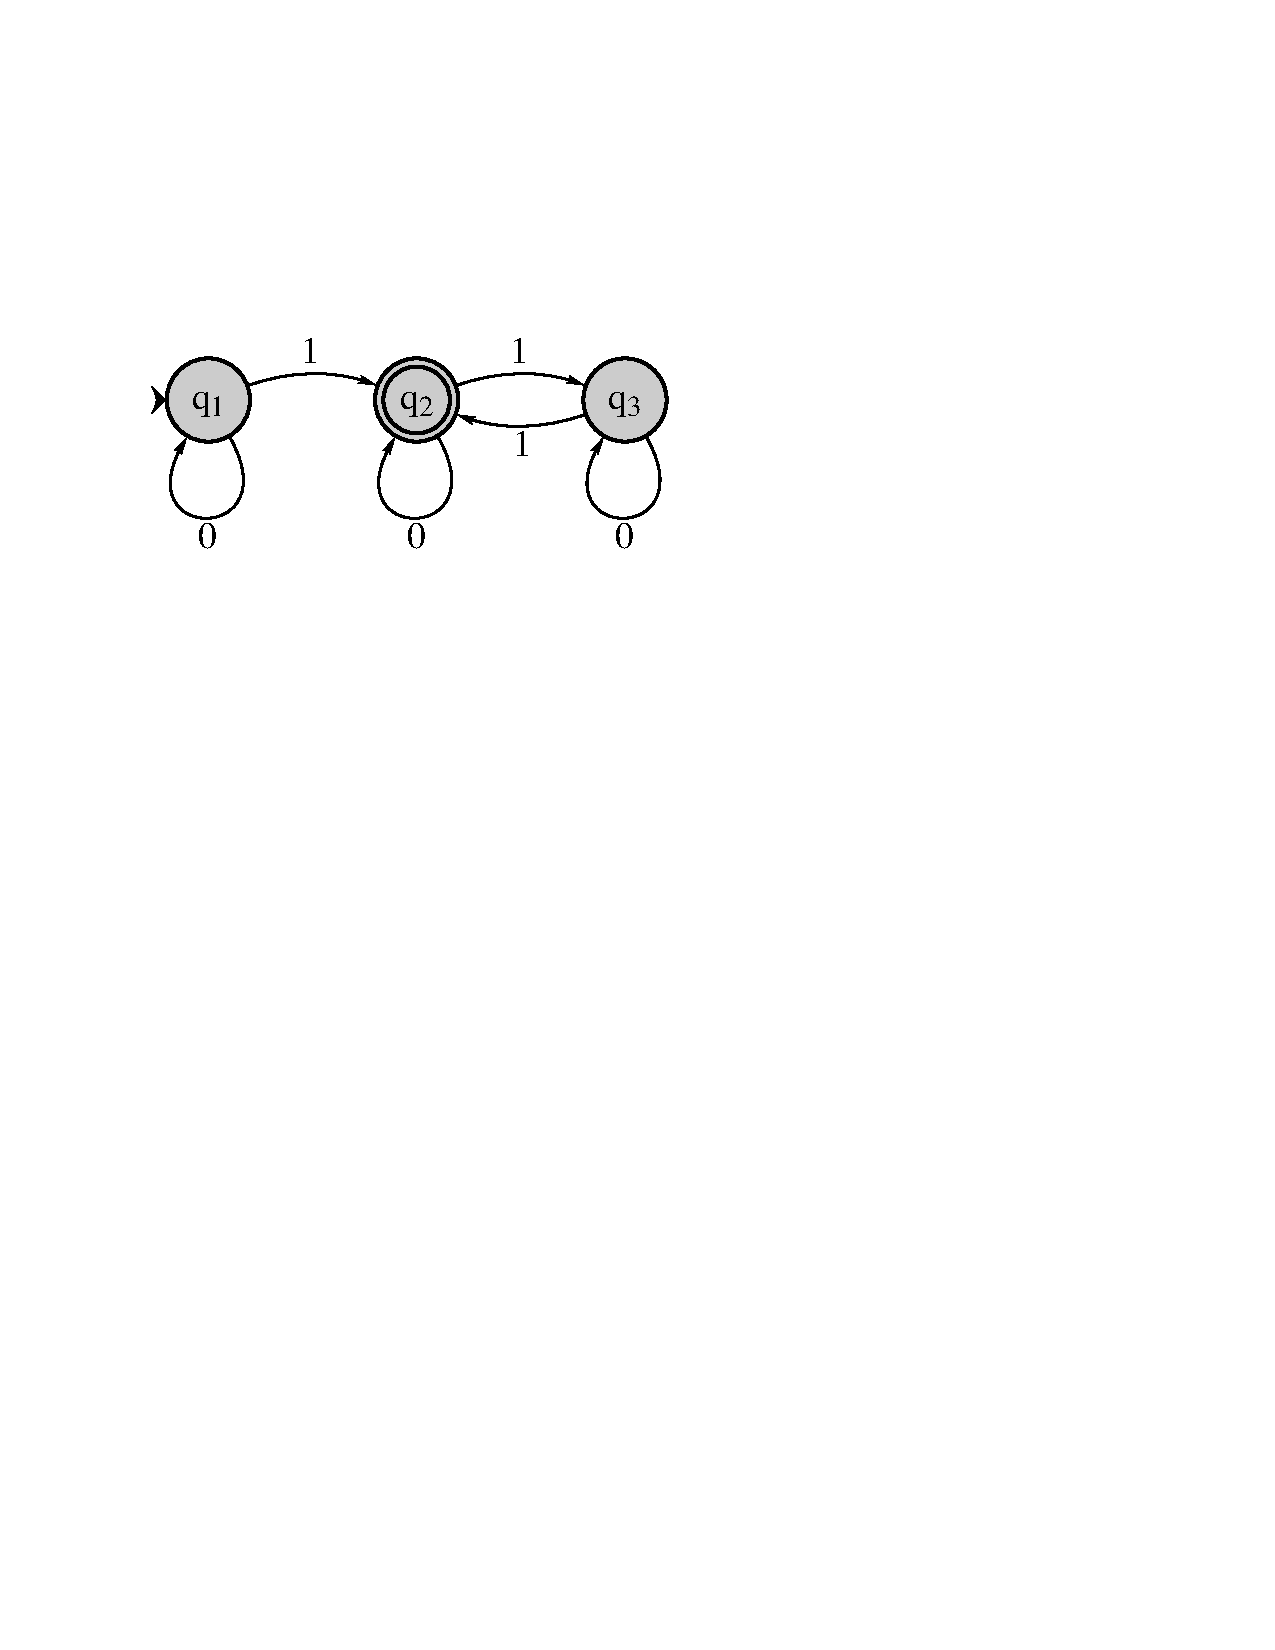
\includegraphics{automin1.pdf}}
\end{center}
\caption{A simple finite automaton}
\label{autom}
\end{figure}
         % Chapter 7, chap7.tex contains an
                        % example of figs and tables and inclusion of pdf.

%%%%%%%%%%%%%%%%%%%%
% Concluding Pages %
%%%%%%%%%%%%%%%%%%%%%%%%%%%%%%%%%%%%%%%%%%%%%%%%%%%%%%%%%%%%%%%%%%%%%%%%%%%%%%%%

% Bibliography or References, REQUIRED

% If using bibtex, create or modify the refs.bib file
% and use (uncomment) the following three lines.
%\bibliographystyle{plain}     
 \bibliographystyle{alpha}
\addcontentsline{toc}{chapter}{\bibname}
\bibliography{refs}         

% If using the ``thereference'' environment instead, modify the ref.tex file
% and use the following line
% ref.tex {References}

\addcontentsline{toc}{chapter}{References}
\begin{thereferences}{99}

\bibitem{Cook1971}
S.~Cook,
 ``The complexity of theorem-proving procedures,''
 {\it Proceedings of the 3rd ACM Symposium on Theory of Computing},
 Shaker Heights, Ohio, 1971, pp.~151--158.

\bibitem{Garey1979}
M.~R.~Garey and D.~S.~Johnson,
 {\it Computers and Intractability: A Guide to the Theory of\/
 {\rm NP}-Completeness},
 W.~H.~Freeman, San Francisco, 1979.

\bibitem{Karp1972}
R.~Karp,
 ``Reducibility among combinatorial problems,''
 in: R.~Miller and J.~Thatcher (eds.),
 {\it Complexity of Computer Computations},
 Plenum Press, New York, 1972, pp.~85--103.

\bibitem{Kearfott1996}
R.~B.~Kearfott and V.~Kreinovich (eds.),
 {\it Applications of Interval Computations},
 Kluwer Academic Publishers, Norwell, MA, 1996.

\bibitem{Kreinovich1993}
V.~Kreinovich, A.~V.~Lakeyev and S.~I.~Noskov,
 ``Optimal solution of interval linear systems is intractable (NP-hard),''
 {\it Interval Computations},
 1993, No. 1, pp. 6--14.

\bibitem{Kreinovich1996a}
 V.~Kreinovich, A.~V.~Lakeyev and J.~Rohn ,
 ``Computational complexity of interval algebraic problems: some are feasible
 and some are computationally intractable: a survey,''
 in: G.~Alefeld and A.~Frommer (eds.),
 {\it Scientific Computing and Validated Numerics},
 Akademie-Verlag, Berlin, 1996, pp.~293--306.

\bibitem{Kreinovich1996b}
 V.~Kreinovich, A.~V.~Lakeyev, J.~Rohn and P.~Kahl,
 {\it Feasible? Intractable? On Computational Complexity of Data Processing
 and Interval Computations},
 Kluwer Academic Publishers, Norwell, MA, 1996 (to appear).

\bibitem{Kulisch1981}
U.~Kulisch and W.~L.~Miranker,
 {\it Computer Arithmetic in Theory and Practice},
 Academic Press, NY, 1981.

\bibitem{Lakeyev1995}
A.~V.~Lakeyev and V.~Kreinovich,
 ``If input intervals are small enough, then interval computations are almost
 always easy,''
 {\it Reliable Computing},
 Supplement (Extended Abstracts of APIC'95: International Workshop on 
 Applications of Interval Computations),
 1995, pp. 134--139.

\bibitem{Levin1973}
L.~Levin,
 ``Universal sequential search problems,''
 {\it Problems of Information Transmission},
 1973, Vol. 9, No. 3, pp. 265--266.

\bibitem{Moore1959}
R.~E.~Moore,
 ``Automatic error analysis in digital computation,''
 {\it Technical Report LMSD-48421},
 Lockheed Missiles and Space Co., Palo Alto, CA, January 1959.

\bibitem{Moore1966}
R.~E.~Moore,
 {\it Interval Analysis},
 Prentice Hall, Englewood Cliffs, NJ, 1966.

\bibitem{Neumaier1990}
A.~Neumaier,
 {\it Interval Methods for Systems of Equations},
 Cambridge University Press, Cambridge, 1990.

\bibitem{Rabinovich1995}
S.~G.~Rabinovich,
 {\it Measurement Errors: Theory and Practice},
 American Institute of Physics, NY, 1995.

\end{thereferences}


% If including appendices, uncomment the following lines,
% adding more includes if needed.
%\StartAppendix
%\include{AppendixA}         % Example of how to include an appendix

% vitae.tex (Curriculum Vitae)

\addcontentsline{toc}{chapter}{Curriculum Vitae}
\chapter*{Curriculum Vitae}

Patrick Thor Kahl was born on July 12, 1961. The first son of Ulf Thor Gustav 
Kahl and Carolyn Kahl, he graduated from Coronado High School, El Paso, Texas, 
in the spring of 1979.  He entered Auburn University in the fall of 1979, and,
in the spring of 1982, The University of Texas at El Paso.  In 1985 he joined
the United States Navy where he served for eight years, most of it aboard the
submarine USS Narwhal (SSN671).  In the fall of 1993, after being honorably
discharged from the navy, Patrick resumed his studies at The University of
Texas at El Paso.  While pursuing his bachelor's degree in Computer Science he
worked as a Teaching Assistant, and as a programmer at the National
Solar Observatory at Sunspot, New Mexico.  He received his bachelor's degree
in Computer Science in the summer of 1994.

In the fall of 1994, he entered the Graduate School of The University of Texas 
at El Paso.  While pursuing a master's degree in Computer Science he worked as 
a Teaching and Research Assistant, and as the Laboratory Instructor for the
1995 Real-Time Programming Seminar at the University of Puerto Rico,
Mayag\"{u}ez Campus.  He was a member of the Knowledge Representation Group
and the Rio Grande Chapter of the Association for Computing Machinery.

\medskip

\noindent
Permanent address: 6216 Sylvania Way

\noindent
\hspace{1.42in}
El Paso, Texas 79912-4927

\vfill

% The following is no longer needed when typed by the author.
%\noindent
%This thesis was typed by <name of typist>.


         % Curriculum Vitae      REQUIRED

%%%%%%%%%%%%%%%%%%%%%%%%%%%%%%%%%%%%%%%%%%%%%%%%%%%%%%%%%%%%%%%%%%%%%%%%%%%%%%%%

\end{document}
